\section{Iteration loop}\label{iteration-loop}

In section \ref{mandelbrot-set} it was mentioned that fractals are calculated
by repeating a formula \emph{iterating} in an iteration loop. The iteration count starts with iteration number 0, at the end of each iteration the count number is increased by 1, then the next iteration of the formula commences (e.g. sequence iters 0, 1, 2, 3, ...). The iterating continues until \emph{termination conditions} are met, which is either when the iteration count equals the \emph{maxiter} or when the \emph({bailout}) condition is achieved.

This section explains the calculations within the iteration loop.

%A fractal formula is built from mathematical equations. These equations can be modifications of the Mandelbrot Set equation (e.g Mandelbulb), and also other mathematical equations.

The equations are made from mathematical operators ($+, -, *, /$) 
and can include functions (e.g. $\sin, \cos, \tan, \exp, \log, sqrt, pow$) 
and also conditions (e.g. if x > y then "run an equation (s)").

A set of equations that have a specific function within the formula are called \emph{transforms}, e.g rotation, scale.

With each iteration of the formula, the point being iterated is \emph{mapped} (moved) to new coordinates as a result of the mathematical equations.  

\subsection{Single formula fractals}\label{single-formula-fractals}

The simplest 3D fractals are calculated by iterating a single fractal formula. More complex fractals are made by iterating a mix of formulas, adding extra transforms, and/or including additional conditions. 

Below there are 3 examples of fractals formulas written in C language code

\subsubsection{Mandelbulb Power 2}\index{Mandelbulb} \nopagebreak

This formula is a modified Mandelbrot Set equation, expanded to \nth{3} dimension.
Cross section at $ z_z = 0 $ looks exactly the same as Mandelbrot Set.
\nopagebreak

\begin{tabular}{l l}
	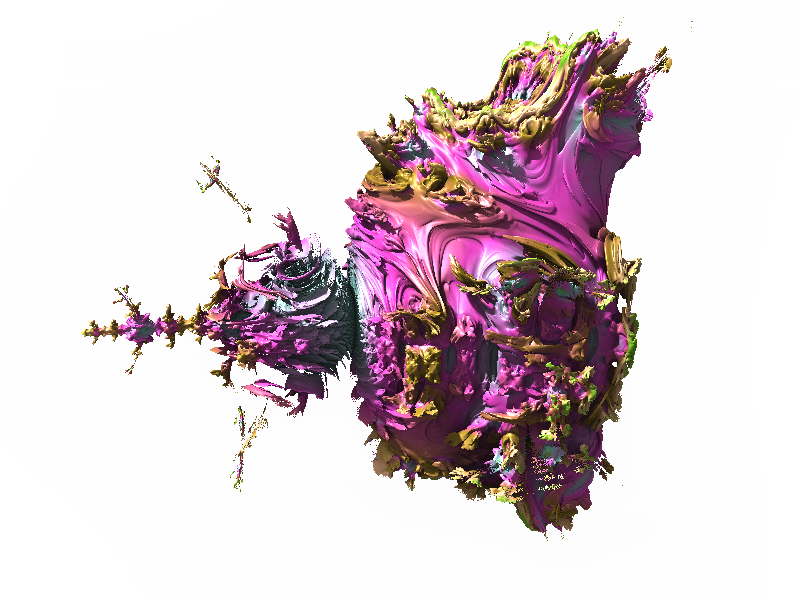
\includegraphics[width=0.3\linewidth]{img/manual/media/formula_mandelbulb_power_2}	
	& 
	\begin{minipage}[b]{0.5\linewidth}
		\begin{verbatim}[fontsize=\scriptsize]
		double x2 = z.x * z.x;
		double y2 = z.y * z.y;
		double z2 = z.z * z.z;
		double temp = 1.0 - z2 / (x2 + y2);
		double newx = (x2 - y2) * temp;
		double newy = 2.0 * z.x * z.y * temp;
		double newz = -2.0 * z.z * sqrt(x2 + y2);
		z.x = newx;
		z.y = newy;
		z.z = newz;
		\end{verbatim}
	\end{minipage}
\end{tabular} 

\subsubsection{Menger Sponge}\index{Menger Sponge} \nopagebreak

This formula is an Iterated Function System (IFS). It contains several
transforms, some of them conditional. \nopagebreak

\begin{tabular}{l l}
	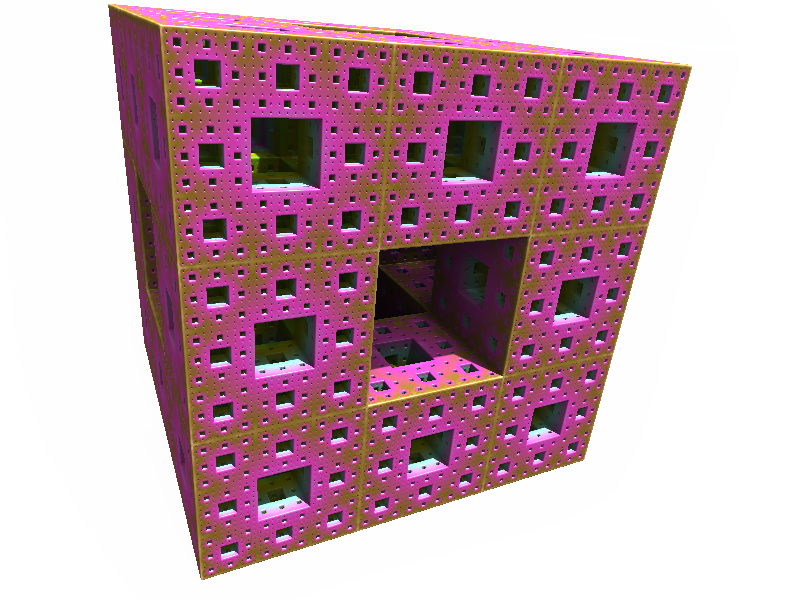
\includegraphics[width=0.3\linewidth]{img/manual/media/formula_menger_sponge.png}	
	& 
	\begin{minipage}[b]{0.5\linewidth}
		\begin{verbatim}[fontsize=\scriptsize]
		z.x = fabs(z.x);
		z.y = fabs(z.y);
		z.z = fabs(z.z);
		
		if (z.x - z.y < 0.0) swap(z.x, z.y);
		if (z.x - z.z < 0.0) swap(z.x, z.z);
		if (z.y - z.z < 0.0) swap(z.y, z.z);
		
		z *= 3.0;
		
		z.x -= 2.0;
		z.y -= 2.0;
		if (z.z > 1.0) z.z -= 2.0;
		\end{verbatim}
	\end{minipage}
\end{tabular} 

\subsubsection{Box Fold Bulb Pow 2}
\nopagebreak

This formula is made from a set of different transforms. It is a good example
how a fractal formula can be more complicated than the
\emph{Mandelbrot Set} formula.

First part is a ``box fold''\index{transform!box fold} transform which conditionally maps the point in x,y,z  directions. Second part is a ``spherical fold''\index{transform!spherical fold} which does conditional scaling in a radial direction.
The end of formula is the same as \emph{Mandelbulb Power 2}. \nopagebreak

\begin{tabular}{l l}
	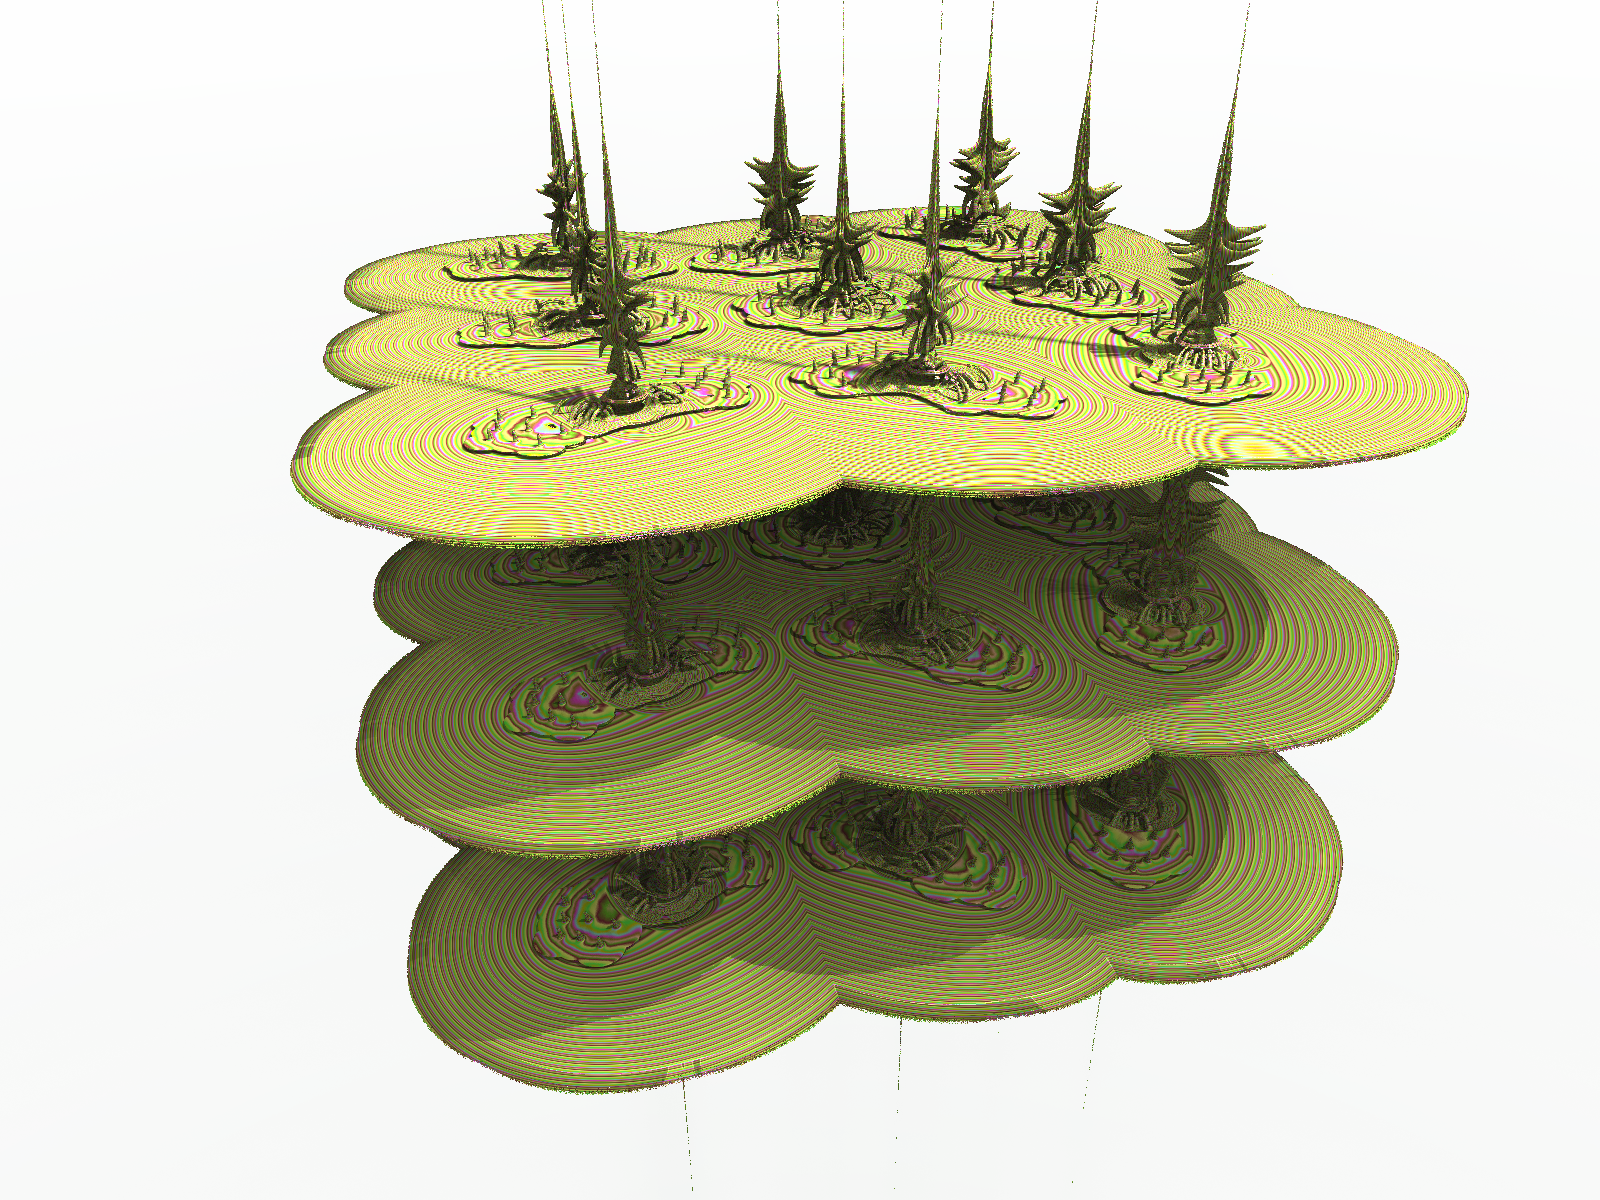
\includegraphics[width=0.3\linewidth]{img/manual/media/formula_box_fold_pwr2.png}	
	& 
	\begin{minipage}[b]{0.5\linewidth}
		\begin{verbatim}[fontsize=\scriptsize]
		//box fold
		if (fabs(z.x) > fractal->foldingIntPow.foldFactor)
		z.x = sign(z.x) * fractal->foldingIntPow.foldFactor * 2.0 - z.x;
		if (fabs(z.y) > fractal->foldingIntPow.foldFactor)
		z.y = sign(z.y) * fractal->foldingIntPow.foldFactor * 2.0 - z.y;
		if (fabs(z.z) > fractal->foldingIntPow.foldFactor)
		z.z = sign(z.z) * fractal->foldingIntPow.foldFactor * 2.0 - z.z;
		
		//spherical fold
		double fR2_2 = 1.0;
		double mR2_2 = 0.25;
		double r2_2 = z.Dot(z);
		double tglad_factor1_2 = fR2_2 / mR2_2;
		
		if (r2_2 < mR2_2)
		{
		z = z * tglad_factor1_2;
		}
		else if (r2_2 < fR2_2)
		{
		double tglad_factor2_2 = fR2_2 / r2_2;
		z = z * tglad_factor2_2;
		}
		
		//Mandelbulb power 2
		z = z * 2.0;
		double x2 = z.x * z.x;
		double y2 = z.y * z.y;
		double z2 = z.z * z.z;
		double temp = 1.0 - z2 / (x2 + y2);
		zTemp.x = (x2 - y2) * temp;
		zTemp.y = 2.0 * z.x * z.y * temp;
		zTemp.z = -2.0 * z.z * sqrt(x2 + y2);
		z = zTemp;
		z.z *= fractal->foldingIntPow.zFactor;
		\end{verbatim}
	\end{minipage}
\end{tabular} 

\subsubsection{Processing of single formula fractals}

Single formula fractals are simply iterated several times until termination conditions are met, as shown in figure \ref{iteration_loops}. \nolinebreak \nopagebreak


\simpleImageWithCaption75Width{img/manual/media/iteration_loops.png}
{Simple Iteration loops with one formula}
{iteration_loops}

When the calculation of the iteration loop finishes the result value of \emph{z} is
used to estimate the distance to the fractal body and to calculate the color of the surface.

\subsection{Hybrid fractals}\index{fractal!hybrid}

It is possible to mix different fractal formulas by alternating their use in the iteration loop.
This way new fractal shapes can be achieved. These fractal combinations are named \emph{hybrid fractals}. 
In the Mandelbulber program there are already many different fractal formulas available which give the user 
the opportunity to use a vast variety of shapes.

\subsubsection{Iteration loop of hybrid fractals}

In general hybrid fractals are calculated in the same way as regular fractals.
The calculation consists of iteration loop, \emph{maxiter} and \emph{bailout} condition. The
difference is in the body of the iteration loop: Instead of one fractal formula there
can be used a different fractal formula in every iteration. The defined
sequence decides in which iteration which formula will be used as the calculation step.
How the sequence will work depends on the following selections:
\begin{itemize}
	\item Which fractal formulas are selected in formula slots
	\item How many iterations are assigned to each formula
	\item Range of iteration numbers where formula will be used
	\item From which fractal slot the sequence will be repeated
\end{itemize}

\simpleImageWithCaption75Width{img/manual/media/iteration_loop_hybrid.png}
{Complex Iteration loop with hybrid fractal}
{iteration_loop_hybrid}

In Mandelbulber it is possible to define nine different fractal formulas which
ca be alternated. Each formula is configured in a separate slot (tab).

\simpleImageWithCaption75Width{img/manual/media/fractal_tabs.png}
{Fractal Tab - Formula only in first slot}
{fractal_tabs}

By default it is possible to setup the fractal formula in the first slot only,
because the program works in single fractal formula mode. There are two ways to
enable hybrid fractals:
\begin{itemize}
	\item Click in any slot with a number higher than one. The program will ask if you want to
	      enable hybrid fractals or boolean mode. Select \emph{Enable hybrid fractals}
	\item Go to \emph{Objects} / \emph{Hybrid} tab. Tick \emph{Enable hybrid fractals} checkbox.
\end{itemize}

After that you can switch to any slot and define fractal formulas in each slot
(if needed) like it's shown in figure \ref{fractal_tabs_with_defined_fractals_tabs_highlighted}.
In this figure \emph{Mandelbulb - Power 2} is selected in slot \#1, \emph{Menger Sponge}
in slot \#2 and \emph{Box Fold Bulb Pow 2} in slot \#3. These formulas will be
used in the next examples.

\simpleImageWithCaption75Width{img/manual/media/fractal_tabs_with_defined_fractals_tabs_highlighted.png}
{Fractal Tab - Multiple formula slots filled}
{fractal_tabs_with_defined_fractals_tabs_highlighted}

\subsubsection{One iteration for each slot}

The simplest way how hybrid fractal can be defined is to use each fractal
formula for only one iteration in the looped sequence.

In figure \ref{iteration_loop_hybrid_sequence_1}, the sequence consists of one \emph{Mandelbulb - Power 2}, one \emph{Menger Sponge} and
one \emph{Box Fold Bulb Pow 2}. The length of the sequence is three, so by every three
iterations the sequencer repeats with the first slot.

\simpleImageWithCaptionFullWidth{img/manual/media/iteration_loop_hybrid_sequence_1.png}
{Hybrid sequence - Simple sequence for three different formulas}
{iteration_loop_hybrid_sequence_1}

This sequence gives a shape which is a mix of properties of all three
formulas, see figure \ref{hybrid_sequence_example_1}.

\simpleImageWithCaptionHalfWidth{img/manual/media/hybrid_sequence_example_1.png}
{Hybrid sequence render - Simple sequence for three different formulas}
{hybrid_sequence_example_1}

Because in the first iteration (slot \#1) \emph{Mandelbulb - Power 2} is used, the general shape
of the fractal is a little similar to \emph{Mandelbulb - Power 2}.

In the next iteration the \emph{Menger Sponge} formula is used. A single iteration
of this formula produces the shape of figure \ref{single_iteration_of_menger_sponge}.

\simpleImageWithCaptionSmallWidth{img/manual/media/single_iteration_of_menger_sponge.png}
{Single iteration of the Menger Sponge}
{single_iteration_of_menger_sponge}

Some properties of this shape are transferred to the generated shape of the hybrid fractal.

\simpleImageWithCaptionHalfWidth{img/manual/media/single_iteration_of_menger_sponge_hybrid.png}
{Hybrid with Menger Sponge features marked in red}
{single_iteration_of_menger_sponge_hybrid}

The Menger sponge shape is distorted, because \emph{Mandelbulb - Power 2} has
already deformed the space.

The third formula \emph{Box Fold Bulb Pow 2} adds leaf-like features to the shape.

\simpleImageWithCaptionSmallWidth{img/manual/media/hybrid_sequence_example_1_leaf_shapes.png}
{Hybrid close up on leaf-like shapes produced by 'Box Fold Bulb Pow 2' formula}
{hybrid_sequence_example_1_leaf_shapes}

\subsubsection{More iterations for each slot}

In each slot it is configurable how many times the fractal formula will be used in the sequence.
On the tab for the given fractal there is parameter \emph{Iterations}.
By default it is set to 1. If this value was increased to 2 on the first and the second tab,
the sequence of formulas are like they are visible in figure \ref{iteration_loop_hybrid_sequence_2}. \label{two-iterations-per-slot}

\simpleImageWithCaptionFullWidth{img/manual/media/iteration_loop_hybrid_sequence_2.png}
{Hybrid sequence - Iteration count on first and second tab set to two}
{iteration_loop_hybrid_sequence_2}

The first and the second formula is repeated twice and the third only once.
The fractal will get the shape in figure \ref{hybrid_sequence_example_2}:

\simpleImageWithCaptionHalfWidth{img/manual/media/hybrid_sequence_example_2.png}
{Hybrid sequence result - Iteration count on first and second tab set to two}
{hybrid_sequence_example_2}

Because \emph{Mandelbulb - Power 2} has two iterations at the beginning, the shape of this formula is more visible.

If the parameter \emph{Iterations} on the second tab is set to 10,
then the \emph{Menger Sponge} formula is used from iteration 2 to iteration 11.

\simpleImageWithCaptionFullWidth{img/manual/media/iteration_loop_hybrid_sequence_3.png}
{Hybrid sequence - Iteration count on second tab set to ten}
{iteration_loop_hybrid_sequence_3}

Like before the initial shape is defined by the first two iterations of \emph{Mandelbulb - Power 2},
but the high number of \emph{Menger Sponge} iterations makes \emph{Menger Sponge} features very well visible.

\simpleImageWithCaptionHalfWidth{img/manual/media/hybrid_sequence_example_3.png}
{Hybrid sequence result - Iteration count on second tab set to ten}
{hybrid_sequence_example_3}

\subsubsection{Range of iterations for slot}

The sequence of fractal formulas can be configured more sophisticated.
It is possible to define a range of iterations on which a given formula will be used.

The second formula slot (\emph{Menger Sponge}) in the sequence of figure \ref{iteration_loop_hybrid_sequence_4} has the range of iterations set to \emph{from 4 to 250}.
On each tab the parameters \emph{Start at iteration} and {Stop at iteration} are used to define this range.

\simpleImageWithCaptionFullWidth{img/manual/media/iteration_loop_hybrid_sequence_4.png}
{Hybrid sequence - Range of iteration set to 4-250 on first tab}
{iteration_loop_hybrid_sequence_4}

During the first pass of the sequence \emph{Menger Sponge} formula could be used at iterations 2 and 3.
Because \emph{Start at iteration} was 4 this formula slot was skipped.
During the second pass of the sequence \emph{Menger Sponge} formula was used at iterations 5 and 6,
because these iterations are inside the defined range of iterations.

The shape of the resulting fractal is visible in figure \ref{hybrid_sequence_example_4}

\simpleImageWithCaptionHalfWidth{img/manual/media/hybrid_sequence_example_4.png}
{Hybrid sequence result - Range of iteration set to 4-250 on first tab}
{hybrid_sequence_example_4}

Because iteration number 2 is \emph{Box Fold Bulb Pow 2} formula the shape of it is much more visible.

\subsubsection{Changed order in sequence}

The order of fractal formulas can be easily changed with the use of the arrow buttons.

\simpleImageWithCaption75Width{img/manual/media/fractal_tabs_with_defined_fractals_arrows.png}
{Fractal tabs with highlighted tab-arrows}
{fractal_tabs_with_defined_fractals_arrows}

Pressing these buttons causes swapping of fractal tabs and by that a swapping of the position inside the sequence.

Example based on first case showed in section \ref{two-iterations-per-slot}:
Swapped \emph{Mandelbulb - Power 2} and \emph{Menger Sponge} gives the sequence of figure \ref{iteration_loop_hybrid_sequence_5}.

\simpleImageWithCaptionFullWidth{img/manual/media/iteration_loop_hybrid_sequence_5.png}
{Hybrid sequence - Swapped tab one and two}
{iteration_loop_hybrid_sequence_5}

As visible in figure \ref{hybrid_sequence_example_5}, the shape of the fractal is completely different.

\simpleImageWithCaptionHalfWidth{img/manual/media/hybrid_sequence_example_5.png}
{Hybrid sequence render - Swapped tab one and two}
{hybrid_sequence_example_5}

Even if the the same fractal formulas are used and in the same number of iterations per slot, the shape strongly depends on the order of the formulas.
Now first \emph{Menger Sponge} formula gives initial shape of fractal and \emph{Mandelbulb - Power 2} only modifies the details.
